%
% Documentation for the Doubly Link List API.
%
% $Author$
% $Date$
% $Revision$
%
% Compile directive:
%  latex Linklist.tex
%  dvips -t letter Linklist.dvi -o Linklist.ps
%
% To make html:
%  latex2html -local_icons -no_images Linklist.tex
%
\documentclass[10pt,letterpaper,titlepage]{article}

\usepackage{graphicx}
\usepackage{color}

\newenvironment{lquote}{\begin{list}{}{}\item[]}{\end{list}}

\pagestyle{plain}

\begin{document}

\title{A Users Guide for the\\
       Doubly Linked List API\\
       Version 1.2.0}
\author{Carl J. Nobile\\
	carl.nobile@gmail.com}
\date{Created: March 28, 1999\\
	Updated: \today}
\maketitle

\pagenumbering{roman}
\section*{Preface}
\addcontentsline{toc}{section}{Preface}
Writing an API for a link list came about after many years of struggling with data storage problems.  I would often write link list code embedded in my application, exposing all of its innards to the application.  This was a nightmare to weed through as the application grew in functionality and complexity.  Often much of the functionality that I would have liked in my application would be too difficult to implement or would be kludged in.  If more than one link list was needed my beard would thin.
\vspace{8pt}

\noindent
This manual documents the implementation and use of the Doubly Linked List API.  A brief overview of the design philosophy and how the data is abstracted will be discussed followed by a thorough explanation of the calling and return mechanism of each function.
\vspace{8pt}

\noindent
I hope it is as useful for you as it has been for me.
\vspace{8pt}
\begin{flushright}
Carl J. Nobile\\
April 1999
\end{flushright}
\newpage

\tableofcontents
\newpage

\pagenumbering{arabic}
\section{Distribution}
This Doubly Linked List can be downloaded from the following sites.  The first site below has a web page dedicated to the API.  All current releases will become available here first.
\vspace{8pt}

\begin{verbatim}
http://tetrasys.homelinux.org
\end{verbatim}
\vspace{8pt}

\noindent
You will also find the API at the following site and its mirrors.
\vspace{8pt}

\begin{verbatim}
ftp://ibiblio.org/pub/linux/lib
\end{verbatim}
\vspace{8pt}

\noindent
Bug reports should go to me at carl.nobile@gmail.com.
\newpage

\section{License}
The Doubly Link List API can now be used with either of the two
following licenses. I have added the Eclipse License because it is
somewhat more business friendly and have kept the Artistic License so
as to not disappoint anybody that may already be satisfied with it.

\subsection{Artistic License}
\begin{center}
\Large			 The``Artistic License''\\
\vspace{8pt}
\Large				Preamble\\
\end{center}
\vspace{4pt}
The intent of this document is to state the conditions under which a Package may be copied, such that the Copyright Holder maintains some semblance of artistic control over the development of the package, while giving the users of the package the right to use and distribute the Package in a more-or-less customary fashion, plus the right to make reasonable modifications.
\vspace{8pt}

\noindent
Definitions:
\begin{lquote}
``Package'' refers to the collection of files distributed by the Copyright Holder, and derivatives of that collection of files created through textual modification.

``Standard Version'' refers to such a Package if it has not been modified, or has been modified in accordance with the wishes of the Copyright Holder as specified below.

``Copyright Holder'' is whoever is named in the copyright or copyrights for the package.

``You'' is you, if you're thinking about copying or distributing this Package.

``Reasonable copying fee'' is whatever you can justify on the basis of media cost, duplication charges, time of people involved, and so on.  (You will not be required to justify it to the Copyright Holder, but only to the computing community at large as a market that must bear the fee.)

``Freely Available'' means that no fee is charged for the item itself, though there may be fees involved in handling the item.  It also means that recipients of the item may redistribute it under the same conditions they received it.
\end{lquote}

\noindent
1. You may make and give away verbatim copies of the source form of the Standard Version of this Package without restriction, provided that you duplicate all of the original copyright notices and associated disclaimers.
\vspace{8pt}

\noindent
2. You may apply bug fixes, portability fixes and other modifications derived from the Public Domain or from the Copyright Holder.  A Package modified in such a way shall still be considered the Standard Version.
\vspace{8pt}

\noindent
3. You may otherwise modify your copy of this Package in any way, provided that you insert a prominent notice in each changed file stating how and when you changed that file, and provided that you do at least ONE of the following:

\begin{lquote}
(a) place your modifications in the Public Domain or otherwise make them Freely Available, such as by posting said modifications to Usenet or an equivalent medium, or placing the modifications on a major archive site such as uunet.uu.net, or by allowing the Copyright Holder to include your modifications in the Standard Version of the Package.

(b) use the modified Package only within your corporation or organization.

(c) rename any non-standard executables so the names do not conflict with standard executables, which must also be provided, and provide a separate manual page for each non-standard executable that clearly documents how it differs from the Standard Version.

(d) make other distribution arrangements with the Copyright Holder.
\end{lquote}

\noindent
4. You may distribute the programs of this Package in object code or executable form, provided that you do at least ONE of the following:

\begin{lquote}
(a) distribute a Standard Version of the executables and library files, together with instructions (in the manual page or equivalent) on where to get the Standard Version.

(b) accompany the distribution with the machine-readable source of the Package with your modifications.

(c) give non-standard executables non-standard names, and clearly document the differences in manual pages (or equivalent), together with instructions on where to get the Standard Version.

(d) make other distribution arrangements with the Copyright Holder.
\end{lquote}

\noindent
5. You may charge a reasonable copying fee for any distribution of this Package.  You may charge any fee you choose for support of this Package.  You may not charge a fee for this Package itself.  However, you may distribute this Package in aggregate with other (possibly commercial) programs as part of a larger (possibly commercial) software distribution provided that you do not advertise this Package as a product of your own.  You may embed this Package's interpreter within an executable of yours (by linking); this shall be construed as a mere form of aggregation, provided that the complete Standard Version of the interpreter is so embedded.
\vspace{8pt}

\noindent
6. The scripts and library files supplied as input to or produced as output from the programs of this Package do not automatically fall under the copyright of this Package, but belong to whomever generated them, and may be sold commercially, and may be aggregated with this Package.  If such scripts or library files are aggregated with this Package via the so-called ``undump'' or ``unexec'' methods of producing a binary executable image, then distribution of such an image shall neither be construed as a distribution of this Package nor shall it fall under the restrictions of Paragraphs 3 and 4, provided that you do not represent such an executable image as a Standard Version of this Package.
\vspace{8pt}

\noindent
7. C subroutines (or comparably compiled subroutines in other languages) supplied by you and linked into this Package in order to emulate subroutines and variables of the language defined by this Package shall not be considered part of this Package, but are the equivalent of input as in Paragraph 6, provided these subroutines do not change the language in any way that would cause it to fail the regression tests for the language.
\vspace{8pt}

\noindent
8. Aggregation of this Package with a commercial distribution is always permitted provided that the use of this Package is embedded; that is, when no overt attempt is made to make this Package's interfaces visible to the end user of the commercial distribution.  Such use shall not be construed as a distribution of this Package.
\vspace{8pt}

\noindent
9. The name of the Copyright Holder may not be used to endorse or promote products derived from this software without specific prior written permission.
\vspace{2pt}

\noindent
10. THIS PACKAGE IS PROVIDED ``AS IS'' AND WITHOUT ANY EXPRESS OR IMPLIED WARRANTIES, INCLUDING, WITHOUT LIMITATION, THE IMPLIED WARRANTIES OF MERCHANTABILITY AND FITNESS FOR A PARTICULAR PURPOSE.

\begin{center}
The End
\end{center}

\subsection{Eclipse License}

Eclipse Public License - v 1.0

THE ACCOMPANYING PROGRAM IS PROVIDED UNDER THE TERMS OF THIS ECLIPSE PUBLIC LICENSE ("AGREEMENT"). ANY USE, REPRODUCTION OR DISTRIBUTION OF THE PROGRAM CONSTITUTES RECIPIENT'S ACCEPTANCE OF THIS AGREEMENT.

1. DEFINITIONS

"Contribution" means:

a) in the case of the initial Contributor, the initial code and documentation distributed under this Agreement, and
b) in the case of each subsequent Contributor:

i) changes to the Program, and

ii) additions to the Program;

where such changes and/or additions to the Program originate from and are distributed by that particular Contributor. A Contribution 'originates' from a Contributor if it was added to the Program by such Contributor itself or anyone acting on such Contributor's behalf. Contributions do not include additions to the Program which: (i) are separate modules of software distributed in conjunction with the Program under their own license agreement, and (ii) are not derivative works of the Program.

"Contributor" means any person or entity that distributes the Program.

"Licensed Patents " mean patent claims licensable by a Contributor which are necessarily infringed by the use or sale of its Contribution alone or when combined with the Program.

"Program" means the Contributions distributed in accordance with this Agreement.

"Recipient" means anyone who receives the Program under this Agreement, including all Contributors.

2. GRANT OF RIGHTS

a) Subject to the terms of this Agreement, each Contributor hereby grants Recipient a non-exclusive, worldwide, royalty-free copyright license to reproduce, prepare derivative works of, publicly display, publicly perform, distribute and sublicense the Contribution of such Contributor, if any, and such derivative works, in source code and object code form.

b) Subject to the terms of this Agreement, each Contributor hereby grants Recipient a non-exclusive, worldwide, royalty-free patent license under Licensed Patents to make, use, sell, offer to sell, import and otherwise transfer the Contribution of such Contributor, if any, in source code and object code form. This patent license shall apply to the combination of the Contribution and the Program if, at the time the Contribution is added by the Contributor, such addition of the Contribution causes such combination to be covered by the Licensed Patents. The patent license shall not apply to any other combinations which include the Contribution. No hardware per se is licensed hereunder.

c) Recipient understands that although each Contributor grants the licenses to its Contributions set forth herein, no assurances are provided by any Contributor that the Program does not infringe the patent or other intellectual property rights of any other entity. Each Contributor disclaims any liability to Recipient for claims brought by any other entity based on infringement of intellectual property rights or otherwise. As a condition to exercising the rights and licenses granted hereunder, each Recipient hereby assumes sole responsibility to secure any other intellectual property rights needed, if any. For example, if a third party patent license is required to allow Recipient to distribute the Program, it is Recipient's responsibility to acquire that license before distributing the Program.

d) Each Contributor represents that to its knowledge it has sufficient copyright rights in its Contribution, if any, to grant the copyright license set forth in this Agreement.

3. REQUIREMENTS

A Contributor may choose to distribute the Program in object code form under its own license agreement, provided that:

a) it complies with the terms and conditions of this Agreement; and

b) its license agreement:

i) effectively disclaims on behalf of all Contributors all warranties and conditions, express and implied, including warranties or conditions of title and non-infringement, and implied warranties or conditions of merchantability and fitness for a particular purpose;

ii) effectively excludes on behalf of all Contributors all liability for damages, including direct, indirect, special, incidental and consequential damages, such as lost profits;

iii) states that any provisions which differ from this Agreement are offered by that Contributor alone and not by any other party; and

iv) states that source code for the Program is available from such Contributor, and informs licensees how to obtain it in a reasonable manner on or through a medium customarily used for software exchange.

When the Program is made available in source code form:

a) it must be made available under this Agreement; and

b) a copy of this Agreement must be included with each copy of the Program.

Contributors may not remove or alter any copyright notices contained within the Program.

Each Contributor must identify itself as the originator of its Contribution, if any, in a manner that reasonably allows subsequent Recipients to identify the originator of the Contribution.

4. COMMERCIAL DISTRIBUTION

Commercial distributors of software may accept certain responsibilities with respect to end users, business partners and the like. While this license is intended to facilitate the commercial use of the Program, the Contributor who includes the Program in a commercial product offering should do so in a manner which does not create potential liability for other Contributors. Therefore, if a Contributor includes the Program in a commercial product offering, such Contributor ("Commercial Contributor") hereby agrees to defend and indemnify every other Contributor ("Indemnified Contributor") against any losses, damages and costs (collectively "Losses") arising from claims, lawsuits and other legal actions brought by a third party against the Indemnified Contributor to the extent caused by the acts or omissions of such Commercial Contributor in connection with its distribution of the Program in a commercial product offering. The obligations in this section do not apply to any claims or Losses relating to any actual or alleged intellectual property infringement. In order to qualify, an Indemnified Contributor must: a) promptly notify the Commercial Contributor in writing of such claim, and b) allow the Commercial Contributor to control, and cooperate with the Commercial Contributor in, the defense and any related settlement negotiations. The Indemnified Contributor may participate in any such claim at its own expense.

For example, a Contributor might include the Program in a commercial product offering, Product X. That Contributor is then a Commercial Contributor. If that Commercial Contributor then makes performance claims, or offers warranties related to Product X, those performance claims and warranties are such Commercial Contributor's responsibility alone. Under this section, the Commercial Contributor would have to defend claims against the other Contributors related to those performance claims and warranties, and if a court requires any other Contributor to pay any damages as a result, the Commercial Contributor must pay those damages.

5. NO WARRANTY

EXCEPT AS EXPRESSLY SET FORTH IN THIS AGREEMENT, THE PROGRAM IS PROVIDED ON AN "AS IS" BASIS, WITHOUT WARRANTIES OR CONDITIONS OF ANY KIND, EITHER EXPRESS OR IMPLIED INCLUDING, WITHOUT LIMITATION, ANY WARRANTIES OR CONDITIONS OF TITLE, NON-INFRINGEMENT, MERCHANTABILITY OR FITNESS FOR A PARTICULAR PURPOSE. Each Recipient is solely responsible for determining the appropriateness of using and distributing the Program and assumes all risks associated with its exercise of rights under this Agreement , including but not limited to the risks and costs of program errors, compliance with applicable laws, damage to or loss of data, programs or equipment, and unavailability or interruption of operations.

6. DISCLAIMER OF LIABILITY

EXCEPT AS EXPRESSLY SET FORTH IN THIS AGREEMENT, NEITHER RECIPIENT NOR ANY CONTRIBUTORS SHALL HAVE ANY LIABILITY FOR ANY DIRECT, INDIRECT, INCIDENTAL, SPECIAL, EXEMPLARY, OR CONSEQUENTIAL DAMAGES (INCLUDING WITHOUT LIMITATION LOST PROFITS), HOWEVER CAUSED AND ON ANY THEORY OF LIABILITY, WHETHER IN CONTRACT, STRICT LIABILITY, OR TORT (INCLUDING NEGLIGENCE OR OTHERWISE) ARISING IN ANY WAY OUT OF THE USE OR DISTRIBUTION OF THE PROGRAM OR THE EXERCISE OF ANY RIGHTS GRANTED HEREUNDER, EVEN IF ADVISED OF THE POSSIBILITY OF SUCH DAMAGES.

7. GENERAL

If any provision of this Agreement is invalid or unenforceable under applicable law, it shall not affect the validity or enforceability of the remainder of the terms of this Agreement, and without further action by the parties hereto, such provision shall be reformed to the minimum extent necessary to make such provision valid and enforceable.

If Recipient institutes patent litigation against any entity (including a cross-claim or counterclaim in a lawsuit) alleging that the Program itself (excluding combinations of the Program with other software or hardware) infringes such Recipient's patent(s), then such Recipient's rights granted under Section 2(b) shall terminate as of the date such litigation is filed.

All Recipient's rights under this Agreement shall terminate if it fails to comply with any of the material terms or conditions of this Agreement and does not cure such failure in a reasonable period of time after becoming aware of such noncompliance. If all Recipient's rights under this Agreement terminate, Recipient agrees to cease use and distribution of the Program as soon as reasonably practicable. However, Recipient's obligations under this Agreement and any licenses granted by Recipient relating to the Program shall continue and survive.

Everyone is permitted to copy and distribute copies of this Agreement, but in order to avoid inconsistency the Agreement is copyrighted and may only be modified in the following manner. The Agreement Steward reserves the right to publish new versions (including revisions) of this Agreement from time to time. No one other than the Agreement Steward has the right to modify this Agreement. The Eclipse Foundation is the initial Agreement Steward. The Eclipse Foundation may assign the responsibility to serve as the Agreement Steward to a suitable separate entity. Each new version of the Agreement will be given a distinguishing version number. The Program (including Contributions) may always be distributed subject to the version of the Agreement under which it was received. In addition, after a new version of the Agreement is published, Contributor may elect to distribute the Program (including its Contributions) under the new version. Except as expressly stated in Sections 2(a) and 2(b) above, Recipient receives no rights or licenses to the intellectual property of any Contributor under this Agreement, whether expressly, by implication, estoppel or otherwise. All rights in the Program not expressly granted under this Agreement are reserved.

This Agreement is governed by the laws of the State of New York and the intellectual property laws of the United States of America. No party to this Agreement will bring a legal action under this Agreement more than one year after the cause of action arose. Each party waives its rights to a jury trial in any resulting litigation.
\newpage

\section{Introduction}
There are many goals to achieve when deciding to write an API.  The functions in the library should be reenterable, easy to include in an application, platform independent, and reasonably flexible with enough functionality to be usable.  These goals can often be contradictory; however, they are achievable with enough forethought and planning.
\vspace{8pt}

\noindent
This package is sufficiently abstracted so that the programmer will neither need to know or care how it is implemented; at least that is the goal I have striven to achieve while writing it.
\vspace{8pt}

\noindent
Within this package is found the: source files written in C; make files for various platforms and compilers; a text script which sets the environment correctly when it runs the demo program created by the make utility; README, INSTALL, and HISTORY text files; Artistic License; and the documentation in \LaTeXe\/ form.
\vspace{8pt}

\noindent
A short overview will follow, discussing the philosophy of how the package works including a rationale of the structure and type definition used in the package.
\vspace{8pt}

\noindent
Then the library itself is broken into six groups: \textbf{initialization}, \textbf{status and state}, \textbf{pointer manipulation}, \textbf{list update}, \textbf{search}, and \textbf{input/output}.

\begin{lquote}
(a) The initialization group handles the creation, initializing, and destruction of the link list.

(b) The status and state group returns various kinds of information about the status of the link list during its operation.

(c) The pointer manipulation group allows the positioning of the current pointer to the head, the tail, or an arbitrary node within the list.

(d) The list update group adds and deletes nodes.

(e) The search group returns the record information based on key data or on the absolute record position.

(f) The input/output group saves or retrieves record data to or from a disk file.
\end{lquote}

\noindent
At this writing there are 29 functions in the library, each one of which is thoroughly explained and examples given when needed.
\newpage

\section{Overview}
When writing tools such as this, one needs to be concerned with how it affects the entire programming environment.  One of the most important aspects of this environment is the problem concerning \emph{namespace} pollution.  To minimize this problem I have used DLL\_ as a prefix to all function names and enumerated \emph{typedef}s.
\vspace{8pt}

\noindent
It is often the case that search criteria will remain the same between queries.  As such, a state table is implemented that passes the current state to the search functions.  There are two functions: one to set and the other to read the state table.
\newpage

\section{Structures}
Most implementations of link lists allocate a single node per record and these nodes are what are linked to each other.  This type of algorithm works well when the link list is embedded in the application code, but not when implementing a link list within an API, because it cannot be made reenterant.
\vspace{8pt}

\noindent
A well written Application Programming Interface (API) requires that the functions contained within it be reenterant and also creates an environment in which the code can be abstracted.  In order to take advantage of these two ideas the Doubly Linked List (hereafter referred to as the DLL) has a three level hierarchy as pictured in the figure.
\vspace{8pt}

\noindent
The first level we will refer to as the ``Top Level Struct''.  All the global data is held by one of these structures and it is allocated once for each incident of the link list.  

\small
\begin{verbatim}

typedef struct list
   {
   Node           *head;         /* pointer to head record */
   Node           *tail;         /* pointer to tail record */
   Node           *current;      /* pointer to current record */
   Node           *saved;        /* pointer to stored record */
   size_t         infosize;      /* size of record incident */
   unsigned long  listsize;      /* number of records in list */
   unsigned long  current_index; /* index value of current record */
   unsigned long  save_index;    /* index value of stored record */
   DLL_Boolean    modified;      /* modified flag (TRUE or FALSE) */
   DLL_SrchOrigin search_origin; /* location a search originates from */
   DLL_SrchDir    search_dir;    /* direction the search proceeds from */
   } List;
\end{verbatim}
\normalsize
\vspace{8pt}

\noindent
At the next level is the ``Node Struct''.  This structure holds the pointer to the actual record data plus the pointers to the next and prior nodes.  It is allocated once for each record structure.

\small
\begin{verbatim}
typedef struct node
   {
   Info        *info;            /* pointer to record data */
   struct node *next;            /* pointer to next node */
   struct node *prior;           /* pointer to prior node */
   } Node;
\end{verbatim}
\normalsize
\vspace{8pt}

%\newpage
\begin{figure}
\begin{center}
\graphicspath{{.}}
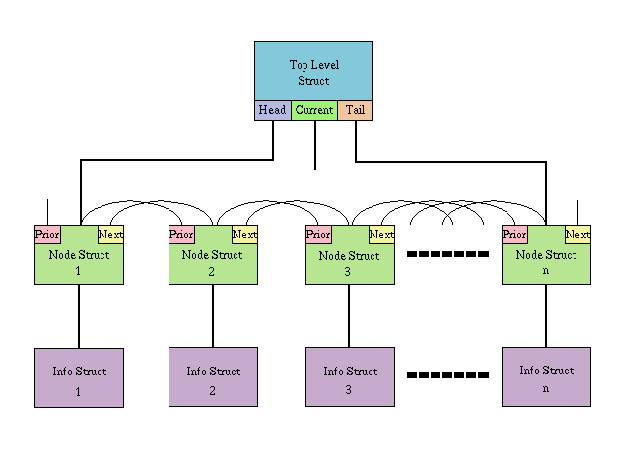
\includegraphics[width=4.75in,hight=4.2in]{linklistDiagram.png}
\vspace{8pt}

Hierarchical Structure of the Doubly Linked List
\end{center}
\end{figure}

\pagebreak
\noindent
The third and final level is the ``Info Struct'', which holds the actual data inserted by the application.  The Info Struct is defined by the developer and is only restricted by the environment in which the application runs or is compiled in.

\small
\begin{verbatim}
typedef struct your_info
   {
   type your_data;               /* Your data goes here */
   } YourInfo;
\end{verbatim}
\normalsize
\vspace{8pt}

\noindent
There is one more structure which is not part of this hierarchy.  It is only used to return the current state of the search criteria.

\small
\begin{verbatim}
typedef struct search_modes
   {
   DLL_SrchOrigin search_origin; /* Search from head, tail, or current */
   DLL_SrchDir    search_dir;    /* Search up or down */
   } DLL_SearchModes;
\end{verbatim}
\normalsize
\newpage

\section{Enumerations}
I'm a firm believer that the return values of functions should be predefined \emph{typedef} enumerations.  There are two reasons for this.  The first is that many compilers will complain when a switch statement is used to test the return values of functions with one or more of the enumerated values missing, thus alerting the developer to use the \emph{default} statement.   The second reason is that the \emph{typedef} name can be used as the return type of the function, disallowing anything other than the enumerated values to be returned.  These are good things and should be taken advantage of.
\vspace{8pt}

\noindent
Since at the time of this writing Booleans are not part of the C specifications, I've created my own.

\small
\begin{verbatim}
typedef enum
   {
   DLL_FALSE,
   DLL_TRUE
   } DLL_Boolean;
\end{verbatim}
\normalsize
\vspace{8pt}

\noindent
Many functions return the \emph{typedef} enumerated type \textbf{DLL\_Return} as shown below.

\small
\begin{verbatim}
typedef enum
   {
   DLL_NORMAL,            /* normal operation */
   DLL_MEM_ERROR,         /* malloc error */
   DLL_ZERO_INFO,         /* sizeof(Info) is zero */
   DLL_NULL_LIST,         /* List is NULL */
   DLL_NOT_FOUND,         /* Record not found */
   DLL_OPEN_ERROR,        /* Cannot open file */
   DLL_WRITE_ERROR,       /* File write error */
   DLL_READ_ERROR,        /* File read error */
   DLL_NOT_MODIFIED,      /* Unmodified list */
   DLL_NULL_FUNCTION      /* NULL function pointer */
   } DLL_Return;
\end{verbatim}
\normalsize
\vspace{8pt}

\noindent
The next two enumerations are used to determine the state of search inquiries: one is used to determine the origin and the other for the direction.  These values are passed as arguments to the \emph{DLL\_SetSearchModes} function.

\small
\begin{verbatim}
typedef enum
   {
   DLL_ORIGIN_DEFAULT,    /* Use current origin setting */
   DLL_HEAD,              /* Set origin to head pointer */
   DLL_CURRENT,           /* Set origin to current pointer */
   DLL_TAIL               /* Set origin to tail pointer */
   } DLL_SrchOrigin;

typedef enum
   {
   DLL_DIRECTION_DEFAULT, /* Use current direction setting */
   DLL_DOWN,              /* Set direction to down */
   DLL_UP                 /* Set direction to up */
   } DLL_SrchDir;
\end{verbatim}
\normalsize
\vspace{8pt}

\noindent
The last enumerated type is used to determine the direction of insertion or the swapping of a record.  This structure is passed as an argument to two functions, \emph{DLL\_InsertRecord} and \emph{DLL\_SwapRecord}.

\small
\begin{verbatim}
typedef enum
   {
   DLL_INSERT_DEFAULT,    /* Use current insert setting */
   DLL_ABOVE,             /* Insert new record ABOVE current record */
   DLL_BELOW              /* Insert new record BELOW current record */
   } DLL_InsertDir;
\end{verbatim}
\normalsize
\newpage

\section{Functions}
The following function calls are grouped by their general functionality, as described above.  They are written in manpage style so that I only have to document the API once.

\subsection{Initialization}
\begin{description}
\item[NAME]\quad\\
DLL\_CreateList, DLL\_InitializeList, DLL\_DestroyList, --- Initialization Functions.

\item[SYNOPSIS]
\begin{verbatim}

#include <linklist.h>

List *DLL_CreateList(List **list);
DLL_Return DLL_InitializeList(List *list, size_t infosize);
void DLL_DestroyList(List **list);
\end{verbatim}

\item[DESCRIPTION]\quad\\
The initialization group of functions must be used in the allocation and freeing of memory used by the link list.

 \begin{description}
 \item[DLL\_CreateList]\quad\\
 This function is called first to create the environment of the link list package.  It is passed \textbf{list}, a pointer to a pointer, of the \emph{Top Level Struct} type \emph{List}.  This pointer is returned both as the return value of the function and in the argument \textbf{list}.

 \item[DLL\_InitializeList]\quad\\
 After defining the \emph{Info} structure this function is called to initialize the environment.  Its first argument, \textbf{list}, is the value returned from \emph{DLL\_CreateList} and the second argument, \textbf{infosize}, is the size in bytes of the \emph{Info} structure.  The value \textbf{DLL\_ZERO\_INFO} is returned if \textbf{infosize} is zero; \textbf{DLL\_NULL\_LIST} if the pointer \textbf{list} is NULL; and \textbf{DLL\_NORMAL} if the initialization was successful.

 \item[DLL\_DestroyList]\quad\\
 Upon exiting the application this function when called will free all memory allocated during this instance of the list.  It is passed \textbf{list}, the value returned from \emph{DLL\_CreateList}, and has no return value of its own; however, the argument \textbf{list} is set to NULL.
 \end{description}

\item[EXAMPLE]
\small
\begin{verbatim}

#include <stdio.h>
#include <stdlib.h>
#include <linklist.h>


typedef struct name_addr    /* Sample data structure */
   {
   char name[30];
   char street[40];
   char city[22];
   char state[3];
   char zip[11];
   } NameAddr;

void main(void)
   {
   List *NAList = NULL;
   DLL_Return DLL_Exit;

   if(DLL_CreateList(&NAList) == NULL)
      {
      fputs("Fatal Memory error", stderr);
      exit(EXIT_FAILURE);
      }

   if((DLL_Exit = DLL_InitializeList(NAList, sizeof(NameAddr)))
    != DLL_NORMAL)
      {
      (void)(DLL_Exit == DLL_ZERO_INFO
       && fputs("Size of address record is zero.\n\n", stderr));
      (void)(DLL_Exit == DLL_NULL_LIST
       && fputs("NAList points to a NULL address.\n\n", stderr));
      exit(EXIT_FAILURE);
      }

   DoYourThingHere(NAList);

   DLL_DestroyList(&NAList);
   exit(EXIT_SUCCESS);
   }
\end{verbatim}
\normalsize

\end{description}
\newpage

\subsection{Status and State}
\begin{description}
\item[NAME]\quad\\
DLL\_Version, DLL\_IsListEmpty, DLL\_IsListFull,\\
DLL\_GetNumberOfRecords, DLL\_SetSearchModes,\\
DLL\_GetSearchModes, DLL\_GetCurrentIndex\\
 --- Status and State Functions.

\item[SYNOPSIS]
\small
\begin{verbatim}

#include <linklist.h>

char *DLL_Version(void);
DLL_Boolean DLL_IsListEmpty(List *list);
DLL_Boolean DLL_IsListFull(List *list);
unsigned long DLL_GetNumberOfRecords(List *list);
DLL_Return DLL_SetSearchModes(List *list, DLL_SrchOrigin origin,
                              DLL_SrchDir dir);
DLL_SearchModes *DLL_GetSearchModes(List *list,
                                    DLL_SearchModes *ssp);
unsigned long DLL_GetCurrentIndex(List *list);
\end{verbatim}
\normalsize

\item[DESCRIPTION]\quad\\
All the functions below except \emph{DLL\_Version} take as their first argument \textbf{list} the pointer returned by \emph{DLL\_CreateList}.  These functions either return or set the status or state of some aspect of the link list.

 \begin{description}
 \item[DLL\_Version]\quad\\
 This function has no arguments and returns a string in the following format:
 \begin{verbatim}
Ver: 1.2.0  June 24 2007
-------------------------------
 Developed by: Carl J. Nobile
Contributions: Charlie Buckheit
               Graham Inchley
               Wai-Sun Chia
 \end{verbatim}
 \vspace{-16pt}
 \item[DLL\_IsListEmpty]\quad\\
 This function determines if the link list has any nodes defined by testing if the head and tail pointers are NULL.  It returns \textbf{DLL\_TRUE} if the list is empty and \textbf{DLL\_FALSE} if the list has valid nodes.

 \item[DLL\_IsListFull]\quad\\
 This function determines if there is enough memory to create new \emph{Node} and \emph{Info} structures by creating and then deleting them.  It returns \textbf{DLL\_TRUE} if either of the two structures could not be allocated and \textbf{DLL\_FALSE} if the memory allocations were successful.

 \item[DLL\_GetNumberOfRecords]\quad\\
 This function returns the number of records currently in the link list by retrieving a counter value.  It returns the number of nodes allocated where a return value of zero is an empty list.

 \item[DLL\_SetSearchModes]\quad\\
 This function sets the search mode state table which is used by various function in the API.  Its second and third arguments are \textbf{origin} and \textbf{dir}.  The \textbf{origin} argument can take one of four values:

  \begin{description}
  \item[DLL\_HEAD] The origin of the search starts from the node which is at the head of the list.  This is the default value if none have been set beforehand.
  \item[DLL\_CURRENT] The origin of the search starts from the currently selected node.
  \item[DLL\_TAIL] The origin of the search starts from the node which is at the tail of the list.
  \item[DLL\_ORIGIN\_DEFAULT] The origin of the search defaults to the last set value.
  \end{description}

 The \textbf{dir} argument can take one of three values:

  \begin{description}
  \item[DLL\_DOWN] The direction of the search is from the head to the tail nodes.  This is the default value if none have been set beforehand.
  \item[DLL\_UP] The direction of the search is from the tail to the head nodes.
  \item[DLL\_DIRECTION\_DEFAULT] The direction of the search defaults to the last set value.
  \end{description}

 It returns \textbf{DLL\_NOT\_MODIFIED} if an invalid value was passed in either \textbf{origin} or \textbf{dir}.  \textbf{DLL\_NORMAL} is returned if the state table was set.

 \item[DLL\_GetSearchModes]\quad\\
 This function gets the state of the search criteria, which can either be the default values or those set by \emph{DLL\_SetSearchModes}.  Its second argument is \textbf{ssp}, a pointer to the structure below.  It returns a pointer to this same instance of the structure.

 \begin{verbatim}
   typedef struct search_modes
      {
      DLL_SrchOrigin search_origin;
      DLL_SrchDir    search_dir;
      } DLL_SearchModes;
 \end{verbatim}

\emph{NOTE: This function has a different argument list starting with release linlkist-1.1.0.  The original function allocated the structure internally to the function, which was not thread safe.  This WILL break old code that used this function.}

 \item[DLL\_GetCurrentIndex]\quad\\
 This function returns the index of the current record by retrieving a counter value.  A return value of zero is an empty list.
 \end{description}

\item[EXAMPLE]\quad\\
Examples of most of these functions can be seen in the source file \emph{dll\_test.c} used in the testing of the link list API.

\end{description}
\newpage

\subsection{Pointer Manipulation}
\begin{description}
\item[NAME]\quad\\
DLL\_CurrentPointerToHead, DLL\_CurrentPointerToTail,\\
DLL\_IncrementCurrentPointer, DLL\_DecrementCurrentPointer,\\
DLL\_StoreCurrentPointer, DLL\_RestoreCurrentPointer\\
  --- Pointer Manipulation Functions.

\item[SYNOPSIS]
\begin{verbatim}

#include <linklist.h>

DLL_Return DLL_CurrentPointerToHead(List *list);
DLL_Return DLL_CurrentPointerToTail(List *list);
DLL_Return DLL_IncrementCurrentPointer(List *list);
DLL_Return DLL_DecrementCurrentPointer(List *list);
DLL_Return DLL_StoreCurrentPointer(List *list);
DLL_Return DLL_RestoreCurrentPointer(List *list);
\end{verbatim}

\item[DESCRIPTION]\quad\\
The \emph{current} pointer in the link list keeps track of the last used node.  In order for this to be of benefit there needs to be a way of controlling where this pointer is located within the list.  These functions allow the repositioning and storing of this pointer during program execution.
\vspace{8pt}

\noindent
All of these functions return the enumerated type \emph{DLL\_Return} and take only one argument \textbf{list} the pointer returned by \emph{DLL\_CreateList}.

 \begin{description}
 \item[DLL\_CurrentPointerToHead]\quad\\
 This function sets the \emph{current} pointer to the head of the list and sets the \emph{index} counter to 1.  A return value of \textbf{DLL\_NULL\_LIST} indicates that the list has no nodes allocated and \textbf{DLL\_NORMAL} indicates that the function succeeded in its task.

 \item[DLL\_CurrentPointerToTail]\quad\\
 This function sets the \emph{current} pointer to the tail of the list and sets the index counter to the \textbf{listsize} counter.  A return value of \textbf{DLL\_NULL\_LIST} indicates that the list has no allocated nodes and \textbf{DLL\_NORMAL} indicates that the function succeeded in its task.

 \item[DLL\_IncrementCurrentPointer]\quad\\
 This function increments the \emph{current} pointer and the \emph{index} counter each by 1.  A return value of \textbf{DLL\_NULL\_LIST} indicates that the list has no allocated nodes, \textbf{DLL\_NOT\_FOUND} indicates that the end of the list has been reached, and \textbf{DLL\_NORMAL} indicates that the function succeeded in its task.

 \item[DLL\_DecrementCurrentPointer]\quad\\
 This function decrements the \emph{current} pointer and the \emph{index} counter each by 1.  A return value of \textbf{DLL\_NULL\_LIST} indicates that the list has no allocated nodes, \textbf{DLL\_NOT\_FOUND} indicates that the beginning of the list has been reached, and \textbf{DLL\_NORMAL} indicates that the function succeeded in its task.

 \item[DLL\_StoreCurrentPointer]\quad\\
 This function stores the \emph{current} pointer and the \emph{index} counter in the \emph{Top Level Struct} for later retrieval.  Only one value can be stored at a time so calling this function again will destroy the first stored pointer and index values.  A return value of \textbf{DLL\_NOT\_FOUND} indicates that the list is empty and \textbf{DLL\_NORMAL} indicates that the function succeeded in its task.

 \item[DLL\_RestoreCurrentPointer]\quad\\
 This function restores the \emph{current} pointer and the \emph{index} counter from the \emph{Top Level Struct}.  Since only one value can be stored at a time, calling this function again will return the last pointer and index values.  A return value of \textbf{DLL\_NOT\_FOUND} indicates that the list is empty and \textbf{DLL\_NORMAL} indicates that the function succeeded in its task.
 \end{description}

\item[EXAMPLE]\quad\\
Examples of most of these functions can be seen in the source file \emph{dll\_test.c} used in the testing of the link list API.

\end{description}
\newpage

\subsection{List Update}
\begin{description}
\item[NAME]\quad\\
DLL\_AddRecord, DLL\_InsertRecord, DLL\_SwapRecord,\\
DLL\_UpdateCurrentRecord, DLL\_DeleteCurrentRecord,\\
DLL\_DeleteEntireList --- List Update Functions.

\item[SYNOPSIS]
\begin{verbatim}

#include <linklist.h>

DLL_Return DLL_AddRecord(List *list, Info *info,
            int (*pFun)(Info *, Info *));
DLL_Return DLL_InsertRecord(List *list, Info *info,
            DLL_InsertDir dir);
DLL_Return DLL_SwapRecord(List *list, DLL_InsertDir dir);
DLL_Return DLL_UpdateCurrentRecord(List *list,
            Info *record);
DLL_Return DLL_DeleteCurrentRecord(List *list);
DLL_Return DLL_DeleteEntireList(List *list);
\end{verbatim}

\item[DESCRIPTION]\quad\\
These functions manipulate the data in the link list.  They all return the enumerated type \emph{DLL\_Return} and take as their first argument, \textbf{list}, the pointer returned by \emph{DLL\_CreateList}.

 \begin{description}
 \item[DLL\_AddRecord]\quad\\
 This function adds a new node and record to the link list.  The second argument is a pointer to the \emph{Info} structure where the new data is stored.  The third argument is a pointer to a function used to sort the insertion of the new data.  The return value of this function is identical to the return value of the \emph{strcmp} function of the standard C library.
 \vspace{8pt}

 Where the return value is
\begin{verbatim}
   less than zero:     arg1 < arg2,

   zero:               arg1 == arg2, or

   greater than zero:  arg1 > arg2.
\end{verbatim}

 Below is an example of this function:

\begin{verbatim}
   int sort_foo(Info *record, Info *compare)
      {
      return(strcmp(rcrd->info_element,
                    cmp->info_element));
      }

\end{verbatim}
 
 If a \emph{NULL} is passed instead of the function pointer no sorting will take place causing the next new node and record to be added to the tail of the list.  A return value of \textbf{DLL\_MEM\_ERROR} indicates that memory could not be allocated and \textbf{DLL\_NORMAL} indicates that the function succeeded in its task.

 \item[DLL\_InsertRecord]\quad\\
 This function adds a new node and record to the link list above or below current record.  The new record will be current after completion.  The second argument is a pointer to the \emph{Info} structure where the new data is stored.  The third argument is passed an enumerated define of type \emph{DLL\_InsertDir}.  

 \small
 \begin{verbatim}
typedef enum
   {
   DLL_INSERT_DEFAULT, /* Use current insert setting */
   DLL_ABOVE,     /* Insert new record ABOVE current record */
   DLL_BELOW      /* Insert new record BELOW current record */ 
   } DLL_InsertDir;
\end{verbatim}
 \normalsize

 In the current version the value \textbf{DLL\_INSERT\_DEFAULT} is not used; it has been included for conformity to other like definitions and possible future expansion.
\vspace{8pt}

\noindent
 The value \textbf{DLL\_NOT\_MODIFIED}, if returned, indicates that a wrong value was passed in the argument \emph{dir}; \textbf{DLL\_MEM\_ERROR} indicates that memory could not be allocated; and \textbf{DLL\_NORMAL} indicates that the function succeeded in its task.

 \item[DLL\_SwapRecord]\quad\\
 This function swaps the current record up or down one place in the list.  The swapped record will remain current after completion.  The second argument is passed the same enumerated define of type \emph{DLL\_InsertDir} as the function \textbf{DLL\_InsertRecord} above.  The value \textbf{DLL\_NOT\_MODIFIED}, if returned, indicates that a value other than the type \emph{DLL\_InsertDir} was passed in the argument \emph{dir}; \textbf{DLL\_NULL\_LIST} indicates that the list is empty and there are no nodes to swap; \textbf{DLL\_NOT\_FOUND} indicates that the current node is either at the head and cannot be swapped above or is at the tail and cannot be swapped below; and \textbf{DLL\_NORMAL} indicates that the function succeeded in its task.

 \item[DLL\_UpdateCurrentRecord]\quad\\
 This function replaces the current data in an \emph{Info} structure with updated data from the application.  The entire structure gets overwritten so all elements in the updating structure will need to be present whether or not they have been changed.  The second argument of this function is passed a pointer to an \emph{Info} structure which contains the updated information.  The value \textbf{DLL\_NULL\_LIST}, if returned, indicates that the list is empty and \textbf{DLL\_NORMAL} indicates that the function succeeded in its task.

 \item[DLL\_DeleteCurrentRecord]\quad\\
 This function deletes the current \emph{Node} and its \emph{Info} structures from the list.  The value \textbf{DLL\_NULL\_LIST}, if returned, indicates that the list is empty and \textbf{DLL\_NORMAL} indicates that the function succeeded in its task.

 \item[DLL\_DeleteEntireList]\quad\\
 This function deletes all the \emph{Node} and \emph{Info} structures from the list.  It does not delete the \emph{Top Level Struct} allowing the application to add new records without having to reinitialize the list again.  The value \textbf{DLL\_NULL\_LIST}, if returned, indicates that the list is empty and \textbf{DLL\_NORMAL} indicates that the function succeeded in its task.
 \end{description}

\item[EXAMPLE]\quad\\
Examples of most of these functions can be seen in the source file \emph{dll\_test.c} used in the testing of the link list API.

\end{description}
\newpage

\subsection{Search}
\begin{description}
\item[NAME]\quad\\
DLL\_FindRecord, DLL\_FindNthRecord, DLL\_GetCurrentRecord,\\
DLL\_GetPriorRecord, DLL\_GetNextRecord -- Search Functions.

\item[SYNOPSIS]
\begin{verbatim}

#include <linklist.h>

DLL_Return DLL_FindRecord(List *list, Info *record,
            Info *match, int (*pFun)(Info *, Info *));
DLL_Return DLL_FindNthRecord(List *list, Info *record,
            unsigned long skip);
DLL_Return DLL_GetCurrentRecord(List *list, Info *record);
DLL_Return DLL_GetPriorRecord(List *list, Info *record);
DLL_Return DLL_GetNextRecord(List *list, Info *record);
\end{verbatim}

\item[DESCRIPTION]\quad\\
These functions retreive data from the list.  They all return the enumerated type \emph{DLL\_Return} and take as their first argument \textbf{list} the pointer returned by \emph{DLL\_CreateList}.

 \begin{description}
 \item[DLL\_FindRecord]\quad\\
 This function returns in its second argument a record found using the criteria passed in its third argument based on the logic of a function passed as its forth argument.  See \textbf{DLL\_SetSearchModes} for setting the search direction and origin.  The form of the passed in function containing the search criteria is the same as that used by the \textbf{DLL\_AddRecord}, but in this case a \emph{NULL} function pointer cannot be passed.  It is shown below for convenience.
 \vspace{8pt}

 Where the return value is
 \begin{verbatim}
   less than zero:     arg1 < arg2,

   zero:               arg1 == arg2, or

   greater than zero:  arg1 > arg2.
 \end{verbatim}

 Below is an example of this function:

 \begin{verbatim}
   int sort_foo(Info *record, Info *compare)
      {
      return(strcmp(rcrd->info_element,
                    cmp->info_element));
      }

\end{verbatim}

  The value \textbf{DLL\_NULL\_FUNCTION}, if returned, indicates that a \textbf{NULL} was passed as the fourth argument; \textbf{DLL\_NULL\_LIST} indicates that the list is empty; \textbf{DLL\_NOT\_FOUND} indicates that a record could not be found; and \textbf{DLL\_NORMAL} indicates that the function succeeded in its task.

 \item[DLL\_FindNthRecord]\quad\\
 This function returns in its second argument the record found by adding the skip value passed in the third argument to the index value of the current record.  The skip value is an \emph{unsigned long} integer.  See \textbf{DLL\_SetSearchModes} for setting the search direction and origin.  The value \textbf{DLL\_NULL\_LIST}, if returned, indicates that the list is empty; \textbf{DLL\_NOT\_FOUND} indicates that a record could not be found in the list or that the \emph{skip} value was out of range; and \textbf{DLL\_NORMAL} indicates that the function succeeded in its task.

 \item[DLL\_GetCurrentRecord]\quad\\
 This function returns in its second argument the current record.  The value \textbf{DLL\_NULL\_LIST}, if returned, indicates that the list is empty and \textbf{DLL\_NORMAL} indicates that the function succeeded in its task.

 \item[DLL\_GetPriorRecord]\quad\\
 This function returns in its second argument the record just prior to the current record.  The value \textbf{DLL\_NULL\_LIST}, if returned, indicates that the list is empty; \textbf{DLL\_NOT\_FOUND} indicates that the current record is at the head of the list and there is no prior record; and \textbf{DLL\_NORMAL} indicates that the function succeeded in its task.

 \item[DLL\_GetNextRecord]\quad\\
 This function returns in its second argument the record just after the current record.  The value \textbf{DLL\_NULL\_LIST}, if returned, indicates that the list is empty; \textbf{DLL\_NOT\_FOUND} indicates that the current record is at the tail of the list and there is no next record; and \textbf{DLL\_NORMAL} indicates that the function succeeded in its task.
 \end{description}

\item[EXAMPLE]\quad\\
Examples of most of these functions can be seen in the source file \emph{dll\_test.c} used in the testing of the link list API.

\end{description}
\newpage

\subsection{Input/Output}
\begin{description}
\item[NAME]\quad\\
DLL\_SaveList, DLL\_LoadList -- Input/Output Functions.

\item[SYNOPSIS]
\begin{verbatim}

#include <linklist.h>

DLL_Return DLL_SaveList(List *list, const char *path);
DLL_Return DLL_LoadList(List *list, const char *path,
            int (*pFun)(Info *, Info *))
\end{verbatim}

\item[DESCRIPTION]\quad\\
These functions are designed to easily write and read the link list data to a disk.  They take advantage of their ability to access the \emph{Top Level Struct} for saving and loading data quickly; however, this will only be useful in limited cases as most implementations will need application specific file formats.  Both return the enumerated type \emph{DLL\_Return} and take as their first argument, \textbf{list}, the pointer returned by \emph{DLL\_CreateList}, and as their second argument, \textbf{path}, a pointer to the file name.

 \begin{description}
 \item[DLL\_SaveList]\quad\\
 This function saves all the \emph{Info} structures including any \emph{NULL} characters in the elements.  The record size is equal to, \textbf{infosize}, the second argument of the \emph{DLL\_InitializeList} function.
\vspace{8pt}

\noindent
  The value \textbf{DLL\_NULL\_LIST}, if returned, indicates that the list is empty; \textbf{DLL\_OPEN\_ERROR} indicates that the file could not be opened for writing; \textbf{DLL\_WRITE\_ERROR} indicates that there was an error while writing to the file meaning that the data in the list should not be trusted; \textbf{DLL\_NOT\_MODIFIED} indicates that the list has not been modified since the last save and no updating to the file was done; and \textbf{DLL\_NORMAL} indicates that the function succeeded in its task.

 \item[DLL\_LoadList]\quad\\
 This function retrieves from a file data based on the same criteria that it was saved with.  See \emph{DLL\_SaveList} above.  The third argument \textbf{pFun} is a pointer to a sorting function the same as can be found in \textbf{DLL\_AddRecord}.  A \emph{NULL} function pointer can be passes if no sorting is needed.
 \vspace{8pt}

 Where the return value is
 \begin{verbatim}
   less than zero:     arg1 < arg2,

   zero:               arg1 == arg2, or

   greater than zero:  arg1 > arg2.
 \end{verbatim}

 Below is an example of this function:

 \begin{verbatim}
   int sort_foo(Info *record, Info *compare)
      {
      return(strcmp(rcrd->info_element,
                    cmp->info_element));
      }
 \end{verbatim}

 
 \end{description}

\item[EXAMPLE]\quad\\
Examples of most of these functions can be seen in the source file \emph{dll\_test.c} used in the testing of the link list API.
\end{description}

\end{document}
